\setcounter{page}{1}
\section*{Zielsetzung}
Im Jahr 1970 gelang es Arthur Ashkin erstmals dielektrische Glassphären mithilfe einer optischen Falle einzufangen und zu bewegen. \cite{Ashkin70} Im weiteren Verlauf seiner Forschung an den Bell Laboratories entwickelte Ashkin daraufhin die auf der Gradientenkraft basierende optische Pinzette.  Mit dieser war es möglich Teilchen in einer Größenordnung zwischen einigen Mikrometern und einzelnen Atomen zu manipulieren. \cite{Ashkin86}\\
Mithilfe der optischen Pinzette wurde es außerdem möglich, die auf Teilchen wirkenden Kräfte bis in den Pikonewtonbereich zu vermessen. Für die Entwicklung der optischen Pinzette, sowie vor allem für deren Anwendung im Bereich der Mikrobiologie wurde Arthur Ashkin 2018 die Hälfte des Nobelpreises verliehen. \cite{nobel}\\
\\
Im vorliegenden Versuch werden mithilfe der optischen Pinzette Experimente an Glas- und Polystyrenkugeln durchgeführt. Ziel ist es dabei die Federkonstante (auch Fallensteifigkeit) der optischen Falle, und die Boltzmannkonstante zu bestimmen. Weiterhin wird die optische Pinzette eingesetzt, um den Transport von Vesikeln durch Aktin-Myosin-Filamente in einer Zwiebelzelle zu untersuchen.\\

\section{Theorie}
\subsection{Grundlagen der optischen Pinzette}
\label{subsec:OptischePinzette}
Die Kraft, welche auf eine Glasspähre mit Mikrometergröße in einem Laserstrahl wirkt, setzt sich aus einem Streu- und einem Gradientenanteil zusammen und kann durch die geometrische Strahlenoptik erklärt werden.
Das eingestrahlte Licht wird durch die Kugel gestreut, wobei ein Impuls auf die Kugel übertragen wird. Die resultierende Kraft wird auch Strahlungsdruck genannt, und wirkt axial entlang der Ausbreitungsrichtung des Laserlichtes.\\
Weiterhin wird auch bei der Brechung und Reflexion des Lichtes an den Grenzflächen zwischen Kugel und umgebendem Medium ein Impuls übertragen. Die daraus resultierende Kraft zeigt in Richtung der maximalen Intensitätsänderung, und wird daher Gradientenkraft genannt. Handelt es sich bei dem einfallenden Strahl um einen stark fokussierten Gaußstrahl, so hat die Gradientenkraft zusätzlich zur lateralen noch eine axiale Komponente, welche in Richtung des Fokuspunkts zeigt. Die Gradientenkräfte sind in Abbildung \ref{fig:gradforce} veranschaulicht.
\begin{figure}[H]
  \centering
  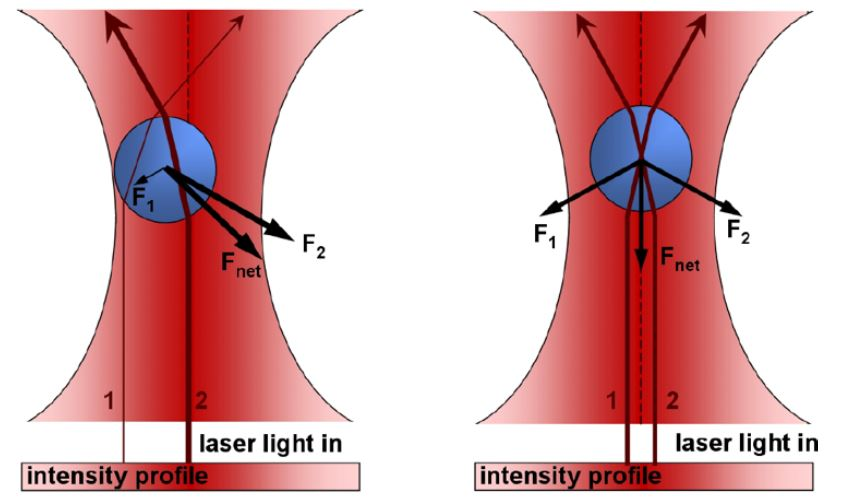
\includegraphics[width=0.65\textwidth]{plots/gradientforce.jpg}
  \caption{Schemazeichnung der auf eine Glasspähre wirkenden optisch induzierten Gradientenkräfte. In \textbf{a)} befindet sich die Kugel ausserhalb der Ruhelage, wodurch eine Kraft Nettokraft hin zum Intensitätsmaximum folg. In \textbf{b)} befindet sich die Kugel in einer lateral stabilen Position. \cite{MIT}}
  \label{fig:gradforce}
\end{figure}
Da die Streukraft und die axiale Gradientenkraft antiparallel zueinander wirken, stellt sich ein Kräftegleichgewicht ein, in dem die Glasspähre gefangen gehalten wird.\\
\\
Für Teilchen, deren Größe deutlich kleiner als die Wellenlänge ist, ist die Näherung über die Strahlenoptik nicht mehr gültig und es muss auf eine Beschreibung durch die Streutheorie nach Rayleigh zurückgegriffen werden. Demnach kann das Teilchen als ein Dipol betrachtet werden und die Streukraft entsteht durch die Absorption und Reemission von Strahlung. Die wirkdende Streukraft kann in der Rayleightheorie von der Gradientenkraft separiert werden, und wird für ein Teilchen mit Radius a durch
\begin{equation}
  F_{\text{sc}} = \frac{I_0\sigma n_m}{c}
\end{equation}
mit der Lichtgeschwindigkeit im Vakuum $c$, der Intensität $I_0$ und dem Brechungsindex des Mediums $n_m$ beschrieben.
Der Streuquerschnitt $\sigma$ für die Streuung von Licht der Wellenlänge $\lambda$ ist gegeben durch
\begin{equation}
  \sigma = \frac{128 \pi^5 a^6}{3\lambda} \left(\frac{m^2-1}{m^2+2}\right)^2 \, .
\end{equation}
Dabei ist $m$ das Verhältnis der Brechungsindizes von Medium und Sphäre.\\
Die Gradientenkraft wird in der Rayleigh Theorie durch die Wechselwirkung eines inhomogenen Lichtfeldes mit dem Dipol beschrieben und zeigt für ein Brechungsindexverhältnis $m>1$ in Richtung des Intensitätsgradienten $\nabla I_0$. \cite{anleitung} Die Gradientenkraft ist mithilfe der Polarisierbarkeit $\alpha$ gegeben durch
\begin{equation}
  F_{\text{grad}} = \frac{2\pi\alpha}{cn_m}\nabla I_0 \,\,\,\,\,\,\, \text{mit} \,\,\,\,\,\,\, \alpha = n_m^2a^3\frac{m^2-1}{m^2+2}\,\,.
\end{equation}

\subsection{Der Zusammenhang von Boltzmannkonstante und Fallensteifigkeit}
Makroskopische Vielteilchensysteme wie Gase und Flüssigkeiten lassen sich durch die Größen Druck $P$, Temperatur $T$ und Volumen $V$ beschreiben.
Der Zusammenhang zwischen der kinetischen Energie des Teilchensystems und dem zugehörigen Druck und Volumen ist im wechselwirkungsfreien Fall durch die ideale Gasgleichung
\begin{equation}
  PV = n k_B T
\end{equation}
gegeben, welche einem $n$-Teilchensystem der Temperatur $T$ in einem Volumen einen makroskopischen Druck zuordnet.
Die dabei auftretende Proportionalitätskonstante ist die Boltzmannkonstante $k_B$, die die Temperatur mit der kinetischen Energie der Teilchen in Beziehung setzt.\\
Da Messgrößen wie die Teilchenzahl eines Gases experimentell nicht zugänglich sind, muss um die Boltzmannkonstante zu messen ein anderer Ansatz gewählt werden. Dieser basiert auf den durch Stöße der Teilchen im Gaß auftretenden Kraftfluktuationen $\langle x \rangle ^2$ und dem Äquipartitionstheorem. Diese Stöße finden zufällig statt und erzeugen die Brownsche Zitterbewegung von Teilchen in einem Umgebungsmedium. Das Theorem besagt, dass auf ein Teilchen im thermischen Gleichgewicht pro Freiheitsgrad die Energie $\frac{1}{2}\k_B T$ entfällt. Außerdem ist die kinetische Energie für ein einzelnes Teilchen in einem harmonischen Potential durch $\frac{1}{2} k \langle x \rangle^2$ festgelegt. Aus dem Gleichsetzen der beiden Terme
folgt
\begin{equation}
  \frac{1}{2}k_B T = \frac{1}{2} k \langle x \rangle^2 \,\,.
\end{equation}
Dabei bezeichnet $k$ die Federkonstante des harmonischen Potentials oder im Falle der optischen Pinzette die Fallensteifigkeit. \cite{anleitung}\\

\subsection{Ermittlung der Boltzmannkonstante über die spektrale Leistungsverteilung}
Die Brownsche Bewegungstheorie gibt neben der Varianz der Teilchenposition $x(t)$ auch Aufschluss über die Verteilung der Positionsfluktuationen des Teilchens. Diese Fluktuationsverteilung kann durch ein Leistungsspektrum beschrieben werden. Dafür wird ein Teilchensystem betrachtet, in dem die Stöße der Teilchen durch eine zufällige Kraft $F(t)$ modelliert werden.
Unter der Annahme, dass die Stöße unkorreliert und die daraus folgenden Korrelationszeiten sehr klein sind, ergibt sich für die Verteilung der Kraft das sogenannte "weisse Rauschen". Die zusätzliche Annahme einer stark gedämpften Teilchenbewegung\footnote{Der Trägheit der gestoßenen Teilchen wirkt als Dämpfung die Viskosität des Umgebungsmediums entgegen. Überwiegen die viskosen Kräfte wird von dem Bereich der kleinen Reynoldszahl gesprochen.} führen auf die Bewegungsgleichung
\begin{equation}
  \beta \dot x(t) + kx(t) = F(t)\, .
\end{equation}
Der hydrodynamische Zugwiderstandswert $\beta = 3\pi\eta d $ setzt sich dabei aus dem Teilchendurchmesser $d$ und der Viskosität $\eta$ zusammen. Zu beachten ist dabei, dass die Federkonstante $k$ unterschiedliche Werte für verschiedene Richtungen aufweisen kann. Mithilfe der Bewegungsgleichung lässt sich so auf die axiale und laterale Steifigkeit der optischen Falle schließen.
Das Leistungsspektrum der Bewegung ergibt sich über das Wiener-Khinchin-Theorem mittels einer Fouriertransfomation der Autokorrelationsfunktion zu
\begin{equation}
  S_{xx} = \sqrt{\frac{k_B T}{\pi^2\beta ( f^2 + f_0^2)}}\, .
\end{equation}
Dabei beinhaltet die \textit{Roll-Off-Frequenz} $f_0 = k / 2\pi\beta$ die Fallensteifigkeit $k$ der optischen Falle. \cite{MIT}\cite{Brown}\\

\subsection{Anwendungen in der Mikrobiologie}
Mithilfe der optischen Pinzette lassen sich auch biologische Vorgänge analysieren. So zum Beispiel die Bewegung von Vesikeln durch Aktin-Myosin Filamente in einer Zwiebelzelle. Bei Vesikeln handelt es sich um Bläschen mit einer Größe von ungefähr $1 \si{\micro\meter}$, deren Außenwand aus Proteinverbindungen bestehen. Die Vesikeln dienen in der Zelle als Transportgefäße für unterschiedliche Stoffe und bewegen sich durch feine Aktin Kanäle. In diesen Kanälen werden die Vesikeln durch Myosin-Motorproteine fortbewegt. Ein Schema des Aufbaus eines Aktin-Myosin Kanals ist in Abbildung \ref{fig:aktin} zu sehen.
\begin{figure}[H]
  \centering
  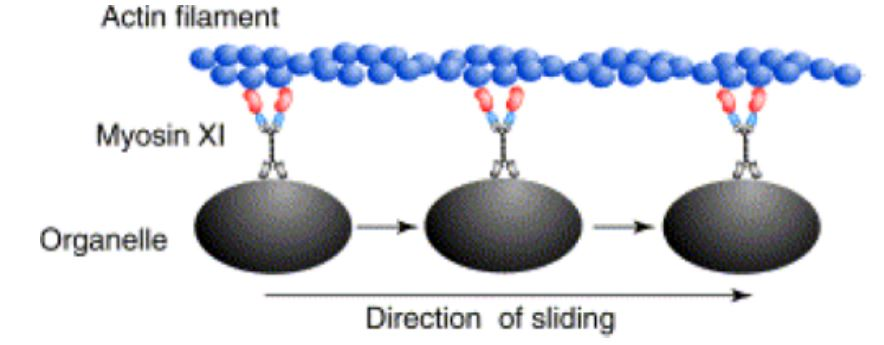
\includegraphics[width=0.5\textwidth]{plots/aktin.jpg}
  \caption{Schemazeichnung der Bewegung eines Vesikels durch einen Aktin-Myosin Kanal. \cite{anleitung}}
  \label{fig:aktin}
\end{figure}
Die Geschwindigkeit der Bewegung, sowie die Reißfestigkeit der Aktin-Filamente kann mithilfe einer optischen Pinzette untersucht werden. \cite{anleitung}
